\documentclass[10pt]{article}

\usepackage{spheric}
%%%TITLE
\title{Analysis of the hydrological safety of dams using numerical tools: Iber and DualSPHysics}
\date{}

%%AFFILIATIONS
\author[$\relax$]{J. Gonz\'alez-Cao$^\dagger$}
\author[$\relax$]{O. Garc{\'\i}a-Feal}
\author[$\relax$]{A.J.C. Crespo}
\author[$\relax$]{J.M. Dom{\'\i}nguez}
\author[$\relax$]{M. G\'{o}mez-Gesteira}
\affil[$\relax$]{Enviromental Physics Laboratory (EPHYSLAB), Universidade de Vigo, Campus As Lagoas, Orense, Spain}
\affil[$\relax$]{\email{\dagger}{ jgcao@uvigo.es}}


%%DOCUMENT
\begin{document}

\maketitle

%\SelectedTopics{}

%%PLEASE PUT YOUR ABSTRACT HERE
\begin{abstract}
The probability of performance failures of the exceedance structures of a dam defines its hydrological safety. These failures are related to water excess in the impoundment of the dam. Recently the failure of the spillways of the Oroville dam (California, USA) forced more than 100000 people to leave their houses. In this work the hydrological safety of Belesar dam is analysed by means of two numerical codes: Iber \cite{crespo2015dualsphysics} and DualSPHysics \cite{blade2014iber}. Iber is a meshbased code that uses the finite volume method to solve the shallow water equations while DualSPHysics is a meshfree code based on SPH methodology that solves the Navier-Stokes equations. The dam (Figure \ref{fig:8-1}) was built in 1962 and it is 127 meters height with a crest 500 meters long. Its impoundment ($\sim$50 km long) is supplied by the hydrological network of the Mi\~{n}o river. The main exceedance structures of the dam are two spillways and four low level outlets. According to the technical specifications, the maximum level of the pool is equal to 330 m and the maximum expected flow of the Mi\~{n}o river is 4000 $\mathrm{m^3/s}$.

\begin{figure}[!htb]
\begin{minipage}[b]{0.42\linewidth}
\centering
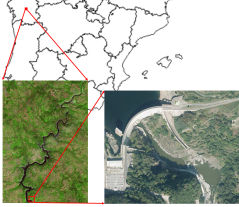
\includegraphics[width=0.8\textwidth]{8-11.png}
\caption{Location of ``Belesar'' dam, impoundment associated to the dam and aerial image of the dam.}\label{fig:8-1}
\end{minipage}
\begin{minipage}[b]{0.05\linewidth}
~
\end{minipage}
\begin{minipage}[b]{0.5\linewidth}
\centering
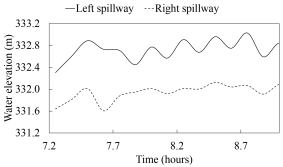
\includegraphics[width=\textwidth]{8-21.png}
\caption{Water elevation close to the dam obtained using Iber.}\label{fig:8-2}
\end{minipage}
\end{figure}
\begin{figure}[!htb]
\begin{minipage}[b]{0.42\linewidth}
\centering
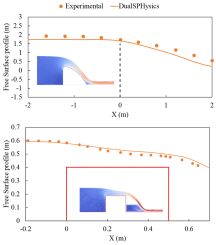
\includegraphics[width=0.8\textwidth]{8-31.png}
\caption{Free surface profile of validation spillways cases obtained with DualSPHysics: ogee spillway (top) and broad crested weir (bottom).}\label{fig:8-3}
\end{minipage}
\begin{minipage}[b]{0.05\linewidth}
~
\end{minipage}
\begin{minipage}[b]{0.5\linewidth}
\centering
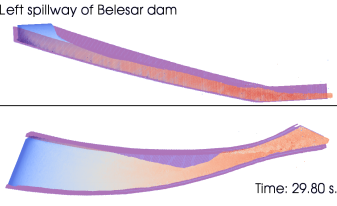
\includegraphics[width=\textwidth]{8-41.png}
\caption{Velocity field of the left spillway of Belesar dam obtained with DualSPHysics.}\label{fig:8-4}
\end{minipage}
\end{figure}

First the water elevation (Figure \ref{fig:8-2}) and the outflow of the spillways associated with the maximum flow of the Mi\~{n}o river were obtained using the numerical code Iber. The numerical domain defined for this simulation uses the real geometry of the dam and its impoundment (obtained from raster files). 

Once the water elevation and the outflow near the spillways were computed, the behaviour of the left spillway of the dam was analysed using the numerical code DualSPHysics. First, two validation cases were considered (Figure \ref{fig:8-3}): an ogee spillway and a broad crested weir. Figure \ref{fig:8-4} shows the velocity field of the left spillway obtained with DualSPHysics.

The main achievement of the present work is the combination of the strengths of Iber and DualSPHysics. Spillways can be simulated starting from the real topography of the impoundment. Iber provides an accurate description of the reservoir that is combined with the capabilities of DualSPHysics to describe extreme flows.






\end{abstract}


%%THE END OF ABSTRACT

\addbib

\end{document}
